\subsection{\bartfull}
\label{subsec:bart}

\bartfull adalah adalah model \ml{} yang dirancang untuk memahami, menghasilkan, dan merekonstruksi teks dalam bahasa alami (\emph{natural language}). \bart{} merupakan \emph{denoising autoencoder} yang dilatih untuk memperbaiki teks yang telah "dirusak" (di-\emph{noise}) oleh berbagai transformasi sehingga mampu mengembalikan teks ke bentuk aslinya \parencite{lewis2019bart}. Arsitektur \bart{} menggabungkan kelebihan model \bert{} yang memiliki \emph{encoder bidirectional} dan GPT yang menggunakan \emph{decoder autoregressive}. Hal ini menjadikannya sangat fleksibel untuk berbagai tugas \nlpfull.

\bart{} dibangun di atas arsitektur transformer yang terdiri atas dua 
komponen utama, yaitu \emph{bidirectional encoder} dan \textit{autoregressive decoder}. 
\emph{Bidirectional encoder} akan mengolah teks input dengan cara memahami hubungan antar token secara dua arah. \emph{Autoregressive decoder} akan menghasilkan teks secara berurutan, token demi token, dengan mempertimbangkan \emph{sequence} yang sudah dihasilkan.

\pagebreak

\begin{figure}
\centering
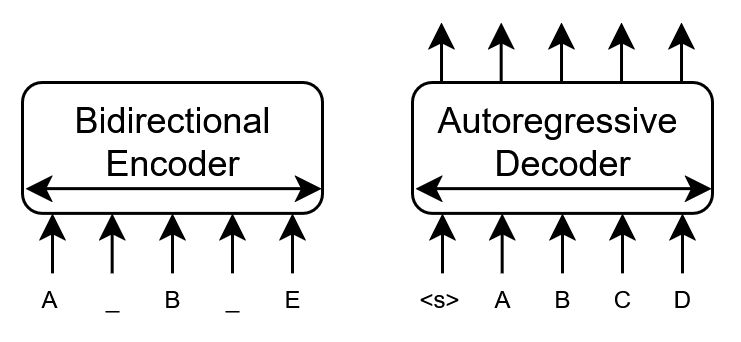
\includegraphics[width=0.8\textwidth]{images/bart.png}
\caption{Cara kerja \bart{} \parencite{lewis2019bart}.}
\label{fig:bart}
\end{figure}

\autoref{fig:bart} menunjukkan cara \bart{} bekerja. Teks input akan “dirusak” terlebih dahulu, kemudian dibaca oleh \encoder. Hasil bacaan \encoder{} akan diteruskan ke \decoder{} untuk mengembalikan bagian teks yang “dirusak” secara 
\textit{autoregressive}. Dengan kemampuannya untuk merekonstruksi teks dari masukan yang rusak, \bart{} menjadi suatu \transformer{} yang sangat baik untuk memahami struktur bahasa dan menghasilkan teks yang koheren walaupun masukan dinilai 
rusak. Penggunaan \bart{} mirip dengan \bert{} dan GPT, seperti klasifikasi teks, generasi teks, dan penejermahan teks. 


